\documentclass[aspectratio=169,11pt]{beamer}
\usepackage[T1]{fontenc}
\usepackage[utf8]{inputenc}
\usepackage[polish]{babel}
\usepackage{booktabs}
\usetheme{default}
\usecolortheme{seahorse}
\setbeamertemplate{navigation symbols}{}
\setbeamertemplate{footline}[frame number]
\graphicspath{{img/}}

\title{System wyszukiwania semantycznego i ekstrakcji wiedzy}
\subtitle{Trzy metody wyszukiwania i NER dla tekstów po polsku}
\author{Eksploracja Danych Tekstowych -- Projekt 2}
\date{2026/2027}

\begin{document}

\begin{frame}
  \titlepage
\end{frame}

\begin{frame}{Aplikacja, korpus i przetwarzanie}
  \begin{columns}[T]
    \column{0.5\textwidth}
    \small
    \textbf{Widoki GUI}
    \begin{itemize}\footnotesize
      \item \textbf{Baza dokumentów}: TXT i PDF, metadane, podgląd z encjami, usuwanie
      \item \textbf{Wyszukiwarka}: 3 metody obok siebie, porównanie kolejności, filtr po encji / typie
      \item \textbf{Encje NER}: wyszukiwanie encji w dowolnej formie, fragmenty, najczęstsze encje
      \item \textbf{Statystyki}: długości, najczęstsze terminy, typy encji
    \end{itemize}
    \textbf{Korpus}
    \begin{itemize}\footnotesize
      \item 40 artykułów z polskiej Wikipedii, 7 tematów, 5 jako PDF (API MediaWiki, CC BY-SA)
      \item 122\,681 słów, ok. 15 tys. wystąpień encji
    \end{itemize}
    \column{0.48\textwidth}
    \small
    \textbf{Przy dodaniu dokumentu:}
    \begin{enumerate}\footnotesize
      \item tekst z TXT / PDF (PyMuPDF)
      \item metadane, wykrycie języka
      \item spaCy \texttt{pl\_core\_news\_md}: lematy bez stopwords + encje (cache)
      \item fragmenty ok. 600 znaków
      \item embeddingi fragmentów (\texttt{multilingual-e5-small})
    \end{enumerate}
    \footnotesize Przy wyszukiwaniu nic nie jest liczone od nowa poza zapytaniem.
  \end{columns}
\end{frame}

\begin{frame}{Trzy metody wyszukiwania}
  \small
  \begin{tabular}{p{0.16\textwidth}p{0.42\textwidth}p{0.32\textwidth}}
    \toprule
    metoda & wynik dokumentu & mocna / słaba strona \\
    \midrule
    słowa kluczowe & dokładne słowa i frazy w cudzysłowie; ranking: ile słów pasuje, potem ile wystąpień
      & dokładne nazwy / nie zna odmiany ani synonimów \\
    TF-IDF & cosinus wektorów TF-IDF z lematów (zapytanie lematyzowane tak samo)
      & odmiana, rzadkie słowa / potrzebne wspólne słowa \\
    semantyczne & max cosinus zapytania do embeddingu fragmentu (\emph{query:} / \emph{passage:})
      & parafrazy / zawsze zwraca $k$ wyników \\
    \bottomrule
  \end{tabular}
  \vspace{0.8em}

  Każda metoda zwraca fragment tekstu związany z zapytaniem. Model semantyczny wybrany
  na 12 zapytaniach: e5-small MRR@5 = 0,96, MiniLM-L12 = 0,82.
\end{frame}

\begin{frame}{Jedno zapytanie -- trzy rankingi}
  \centering
  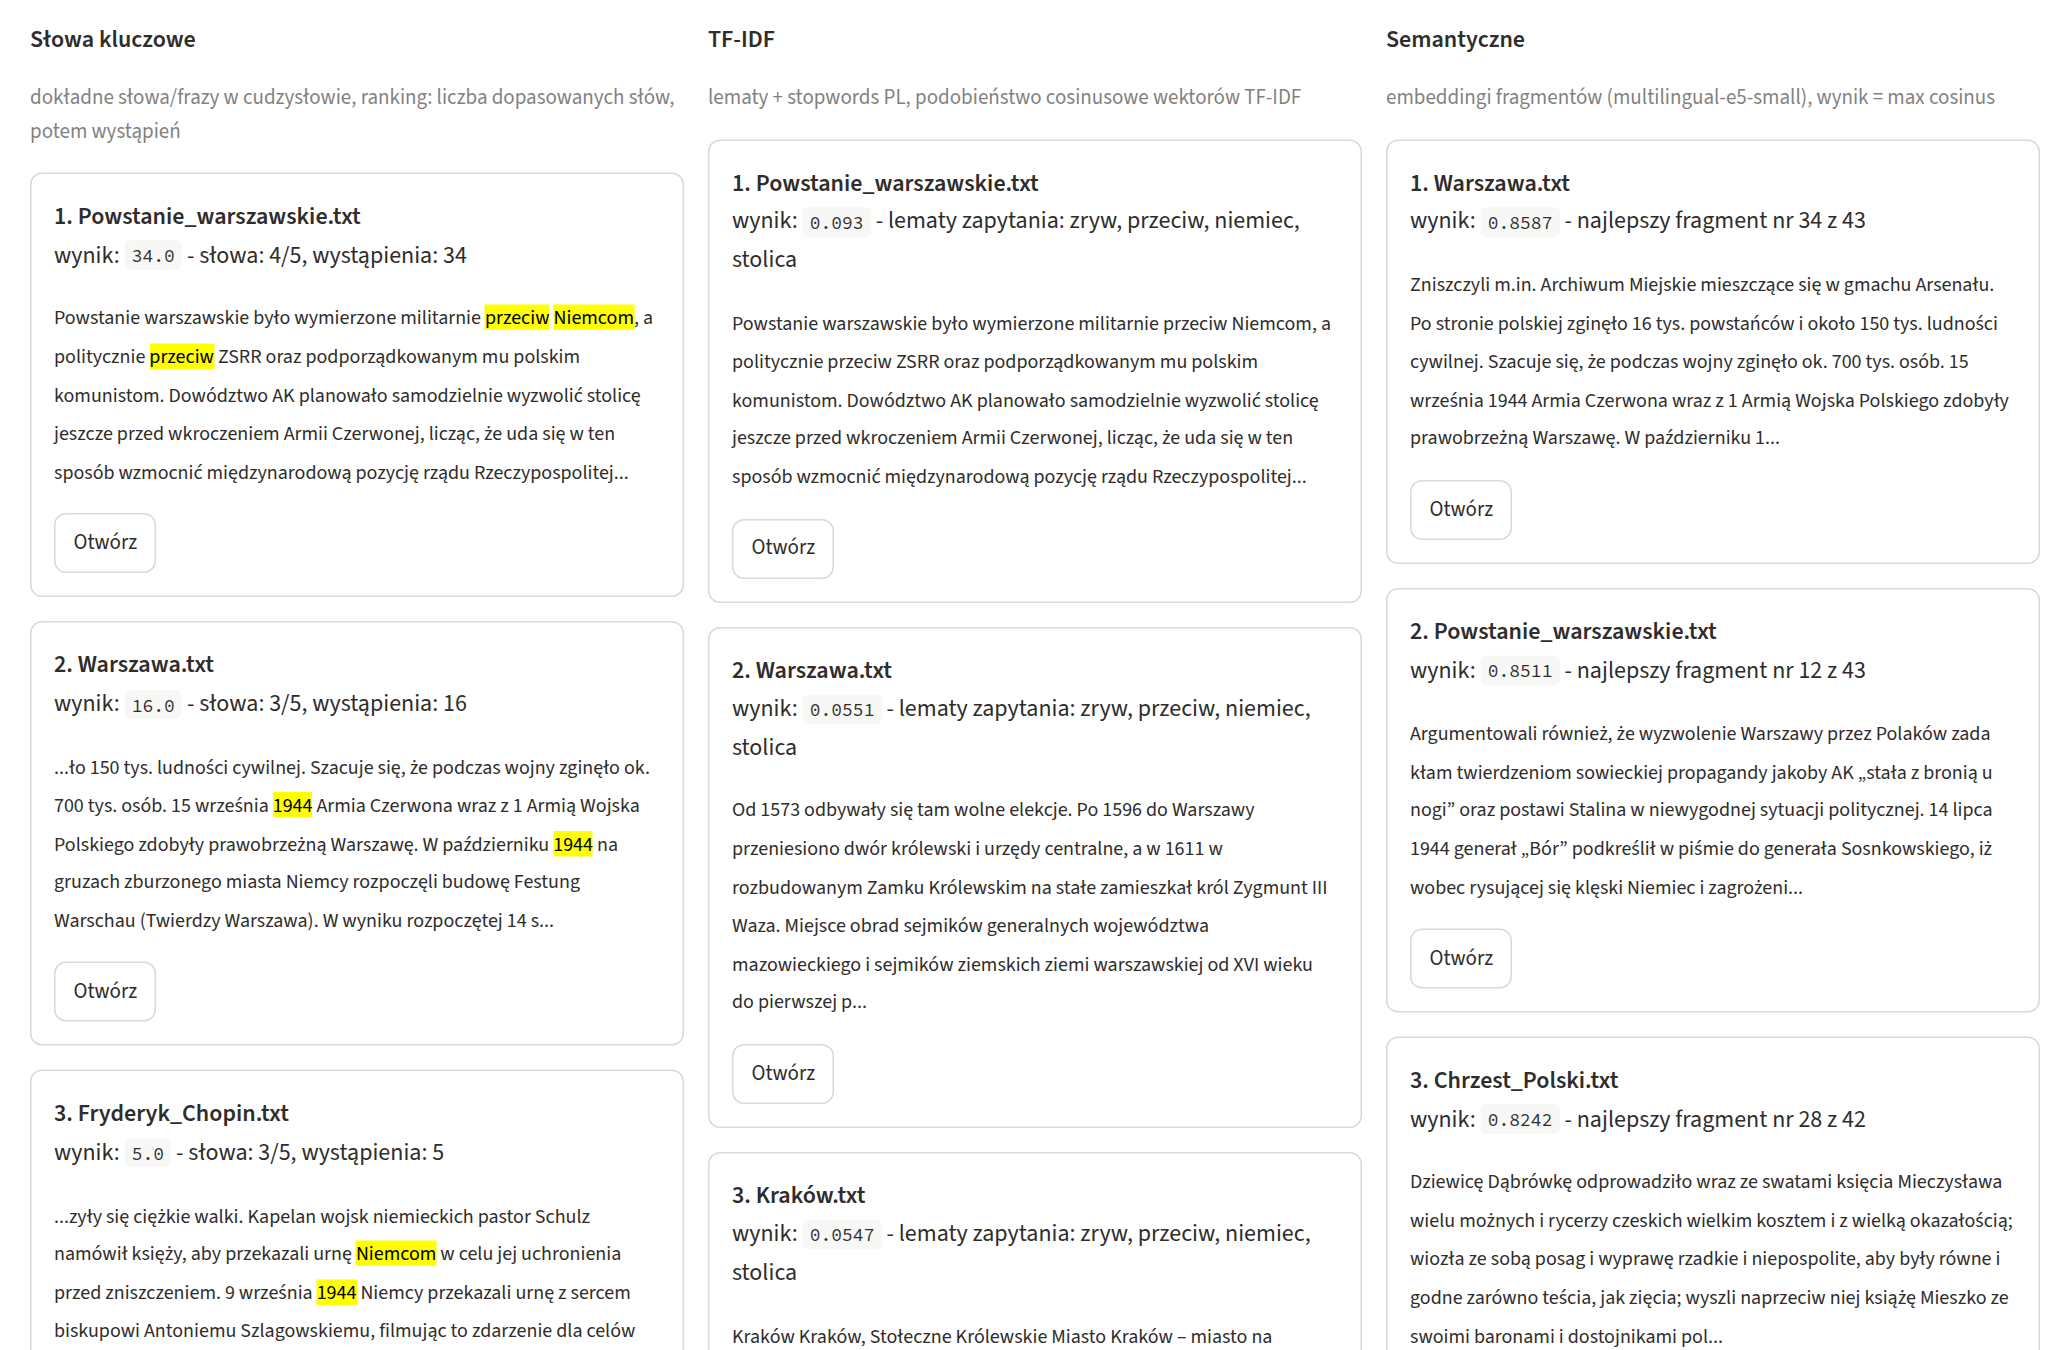
\includegraphics[height=0.84\textheight]{p2_gui_wyniki.png}
\end{frame}

\begin{frame}{Porównanie kolejności dokumentów}
  \begin{columns}[T]
    \column{0.62\textwidth}
    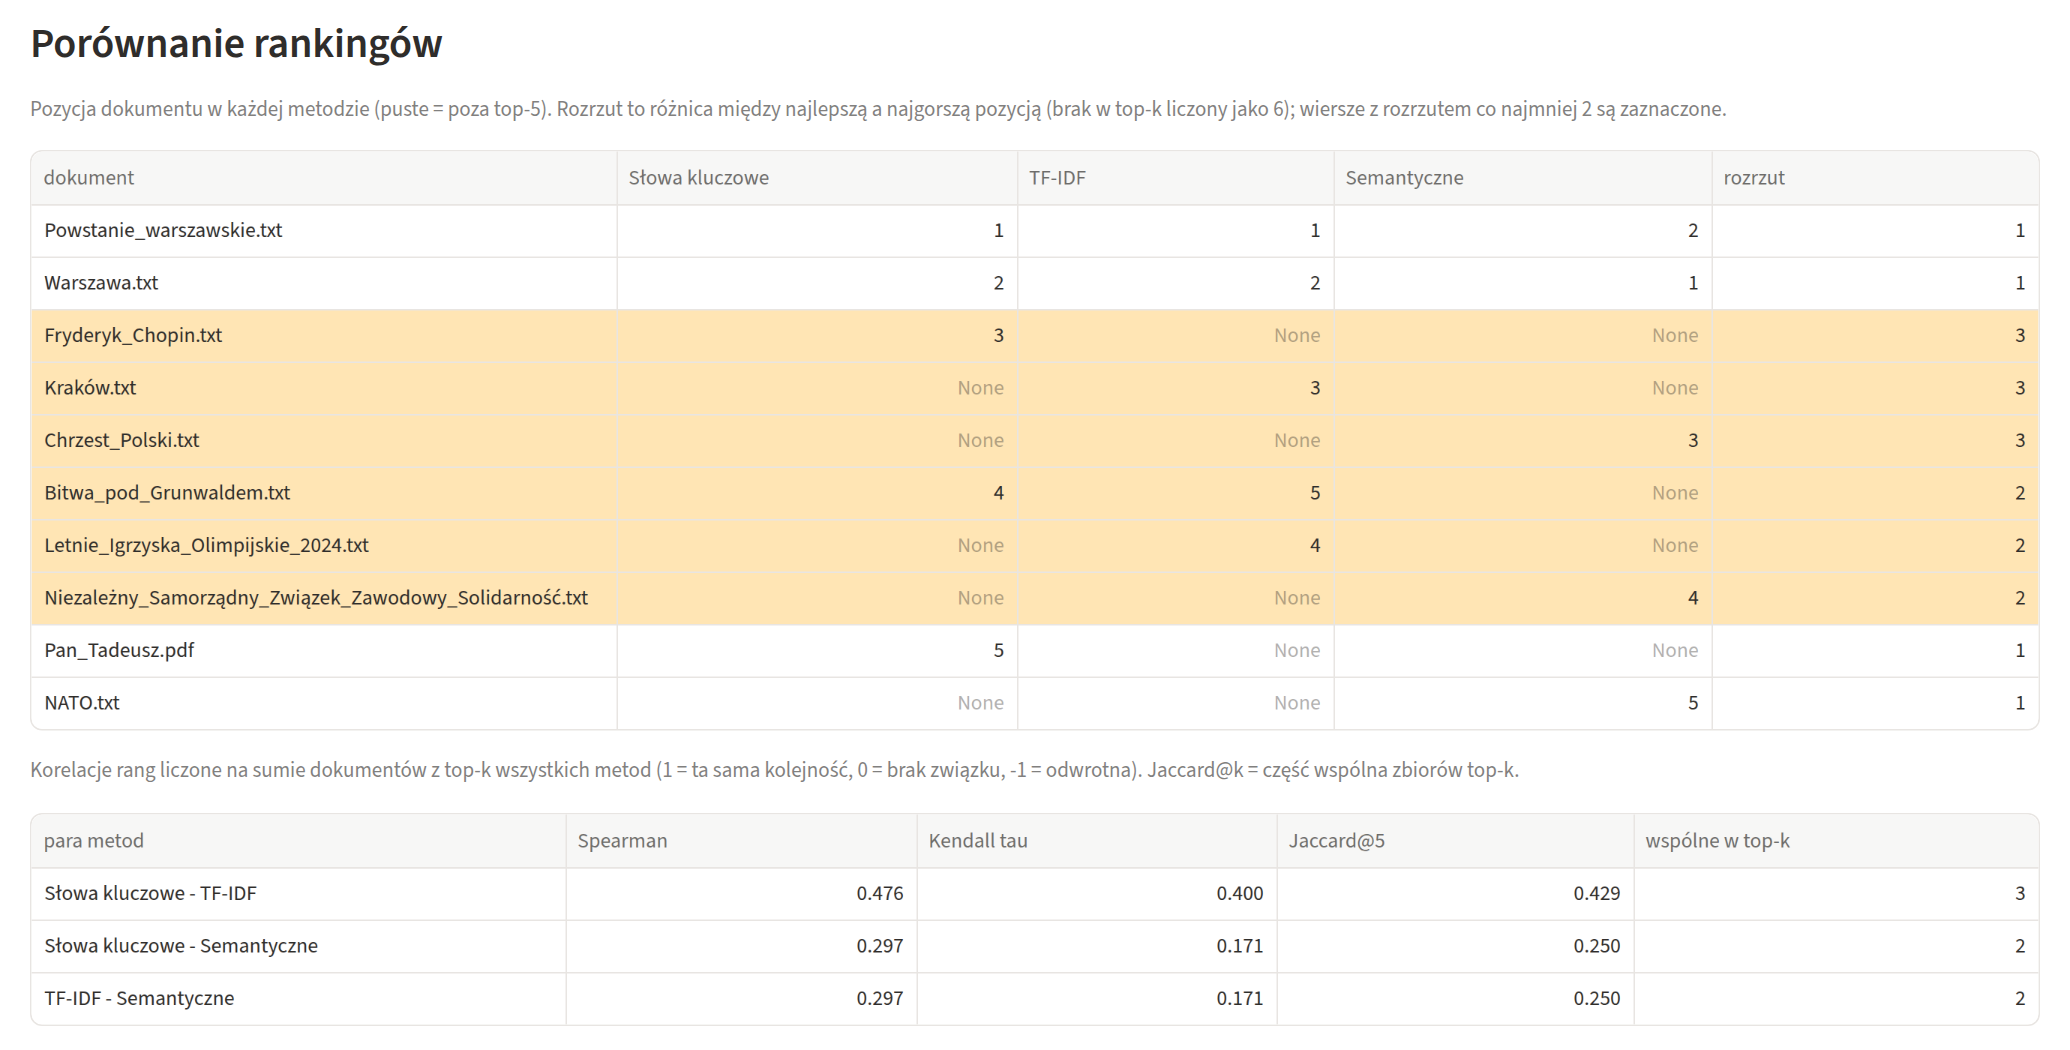
\includegraphics[width=\textwidth]{p2_gui_ranking.png}
    \column{0.36\textwidth}
    \small
    \begin{itemize}
      \item pozycja w każdej metodzie, rozrzut (wyróżnione $\geq 2$)
      \item Spearman i Kendall $\tau$ na sumie top-$k$; brak w top-$k$ $\rightarrow$ pozycja $k+1$
      \item Jaccard@$k$ = $|A \cap B| / |A \cup B|$
    \end{itemize}
  \end{columns}
\end{frame}

\begin{frame}{Eksperyment: 13 zapytań testowych}
  \begin{columns}[T]
    \column{0.5\textwidth}
    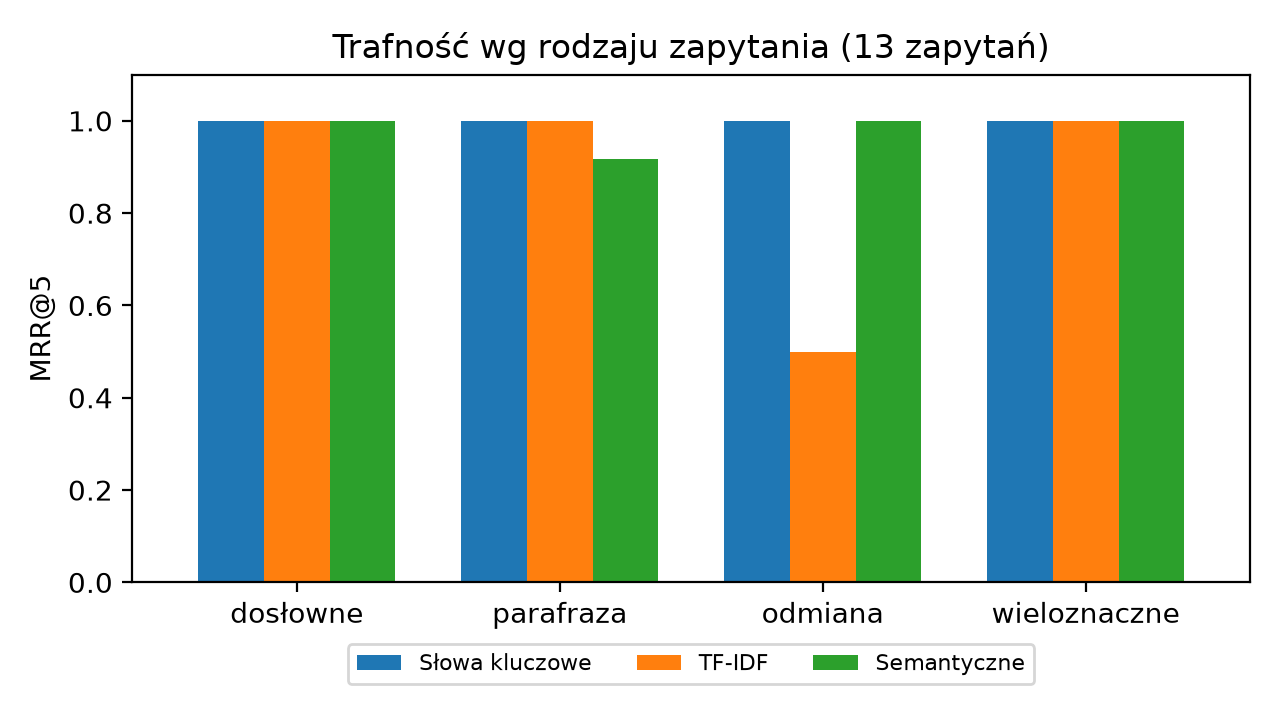
\includegraphics[width=\textwidth]{mrr.png}
    \column{0.5\textwidth}
    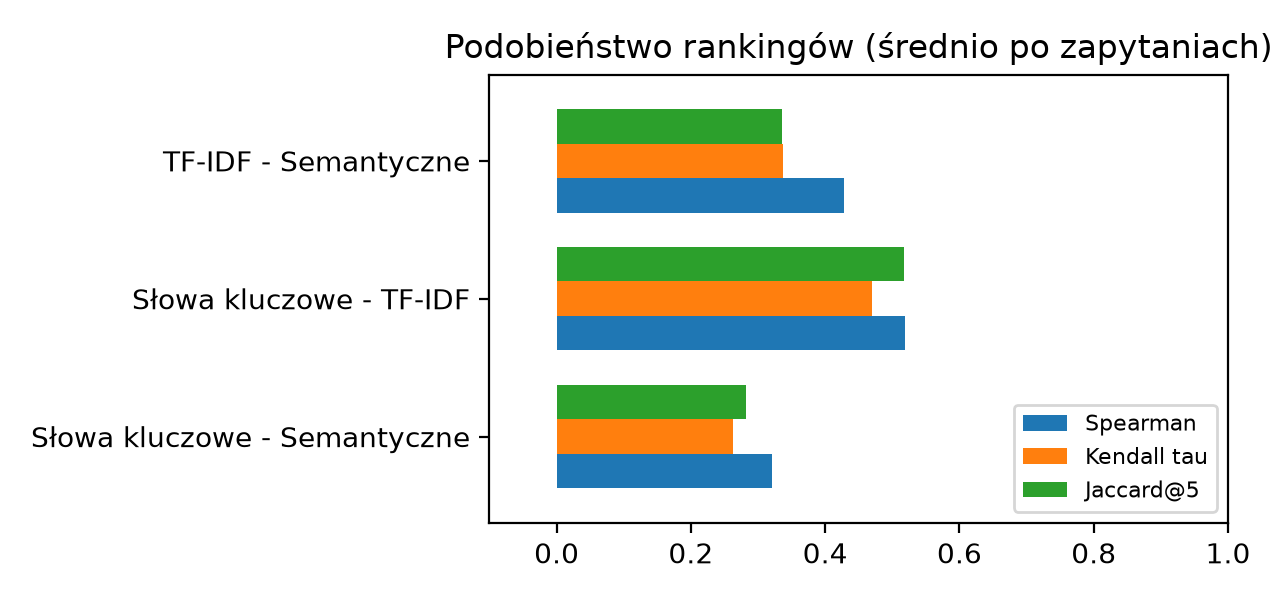
\includegraphics[width=\textwidth]{korelacje.png}
  \end{columns}
  \small
  \begin{itemize}
    \item trafny dokument zwykle na 1. miejscu we wszystkich metodach, ale dalsza kolejność bardzo się różni
    \item TF-IDF przegrywa na ,,Krzyżacy'' -- błędny lemat ze spaCy
  \end{itemize}
\end{frame}

\begin{frame}{NER: wyszukiwanie encji}
  \begin{columns}[T]
    \column{0.62\textwidth}
    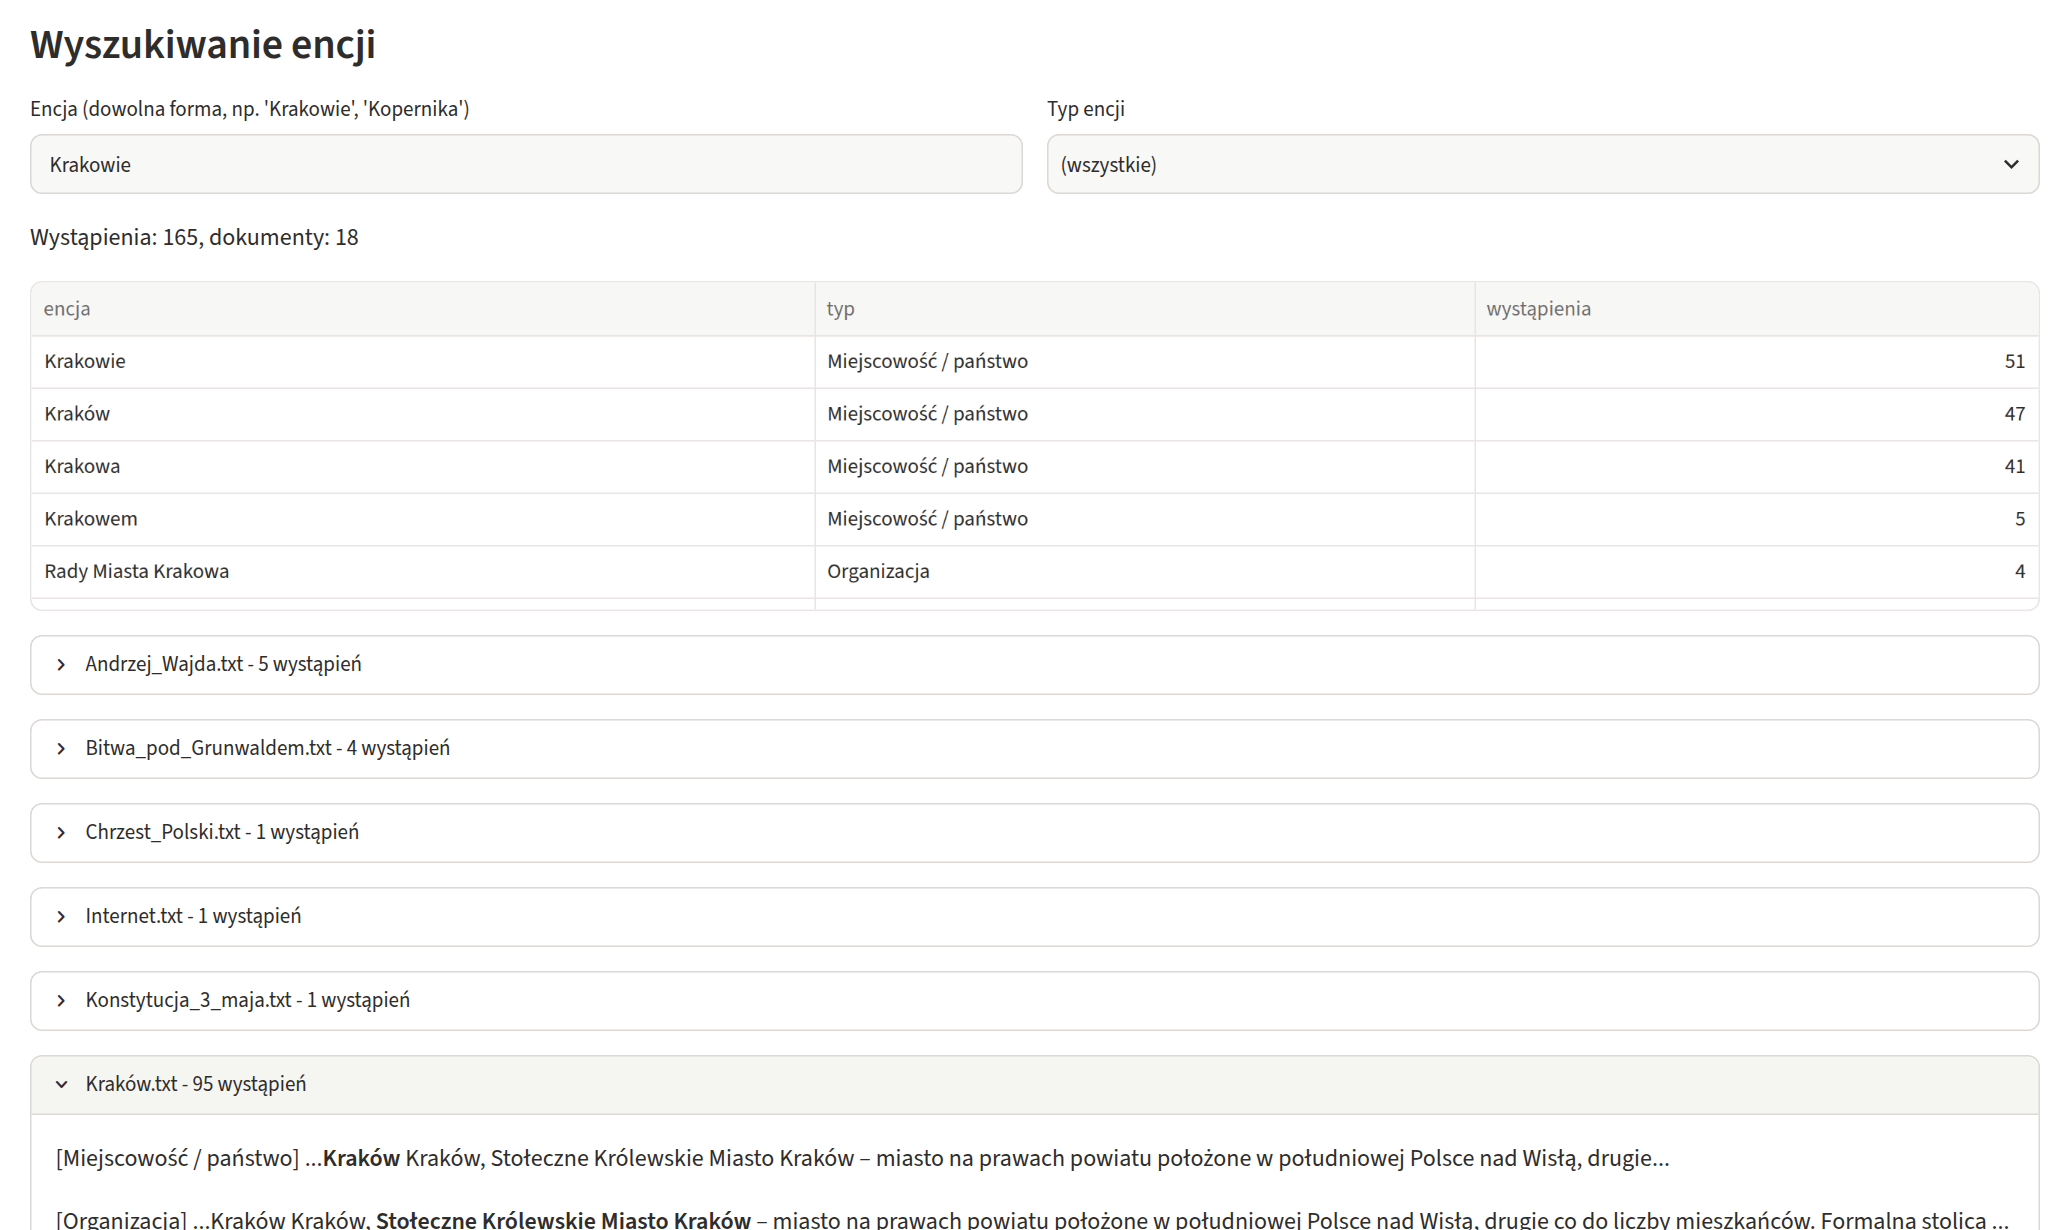
\includegraphics[width=\textwidth]{p2_gui_encje.png}
    \column{0.36\textwidth}
    \small
    \begin{itemize}
      \item typy: osoba, organizacja, miejscowość/państwo, obiekt geograficzny, data, czas
      \item porównanie po lemacie: ,,Krakowie'' znajduje ,,Kraków'', ,,Krakowa'', ,,Krakowem''
      \item lista dokumentów i fragmenty z wyróżnioną encją
    \end{itemize}
  \end{columns}
\end{frame}

\begin{frame}{Filtr encji w wyszukiwarce}
  \centering
  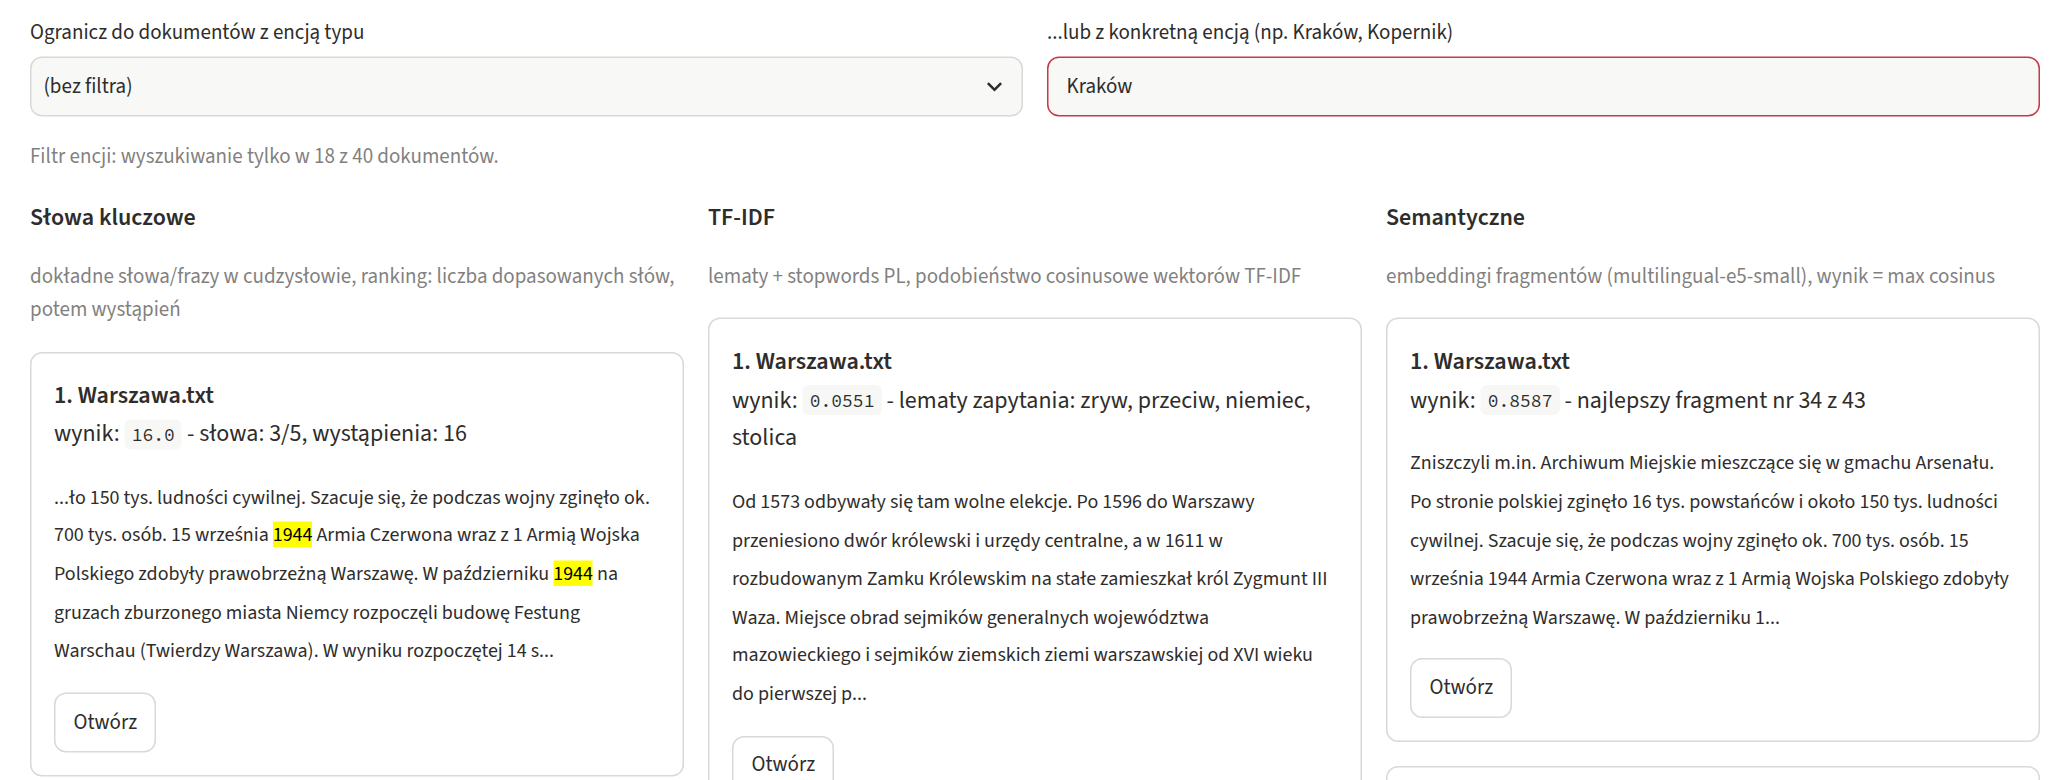
\includegraphics[width=0.9\textwidth]{p2_gui_filtr.png}\\[0.3em]
  \small To samo zapytanie co wcześniej, ale tylko w dokumentach z encją ,,Kraków'' (18 z 40):
  artykuł o powstaniu warszawskim odpada, na 1. miejscu jest Warszawa.
\end{frame}

\begin{frame}{Dokument z encjami, najczęstsze encje, statystyki}
  \begin{columns}[T]
    \column{0.5\textwidth}
    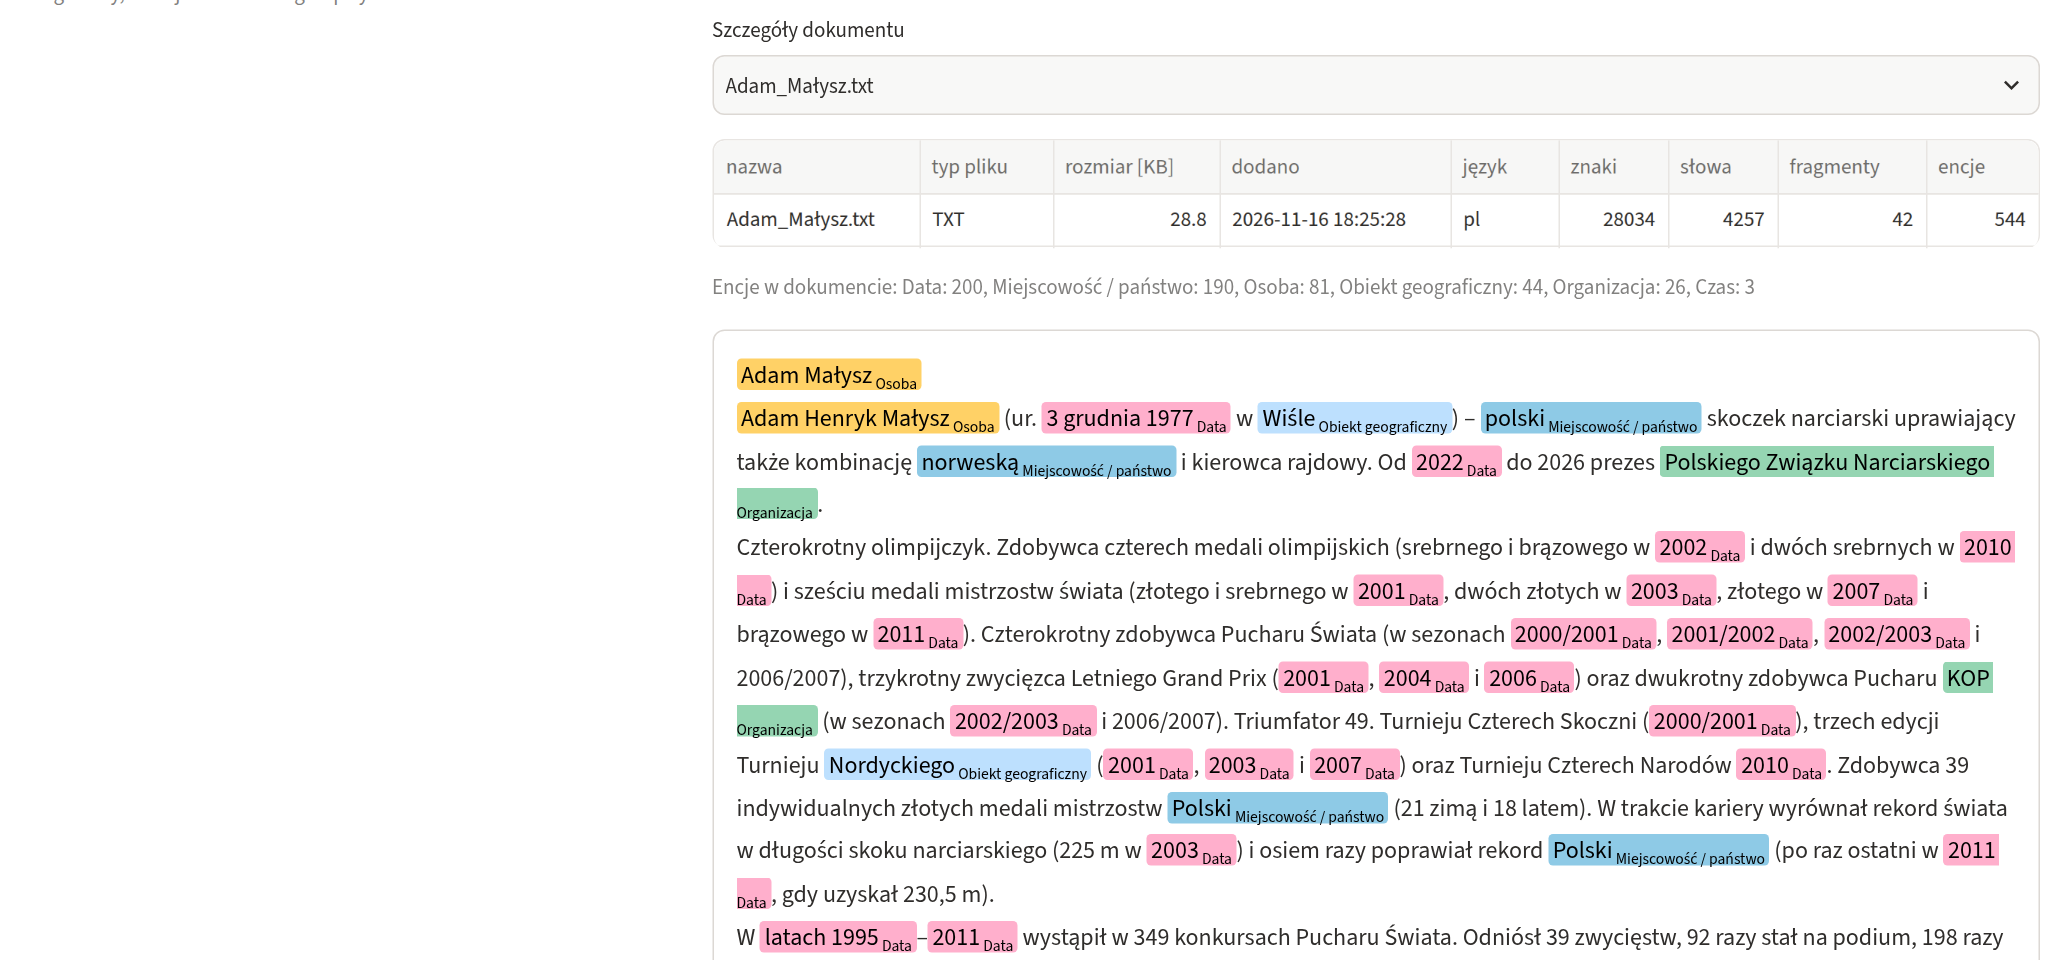
\includegraphics[width=\textwidth]{p2_gui_dokument.png}
    \column{0.5\textwidth}
    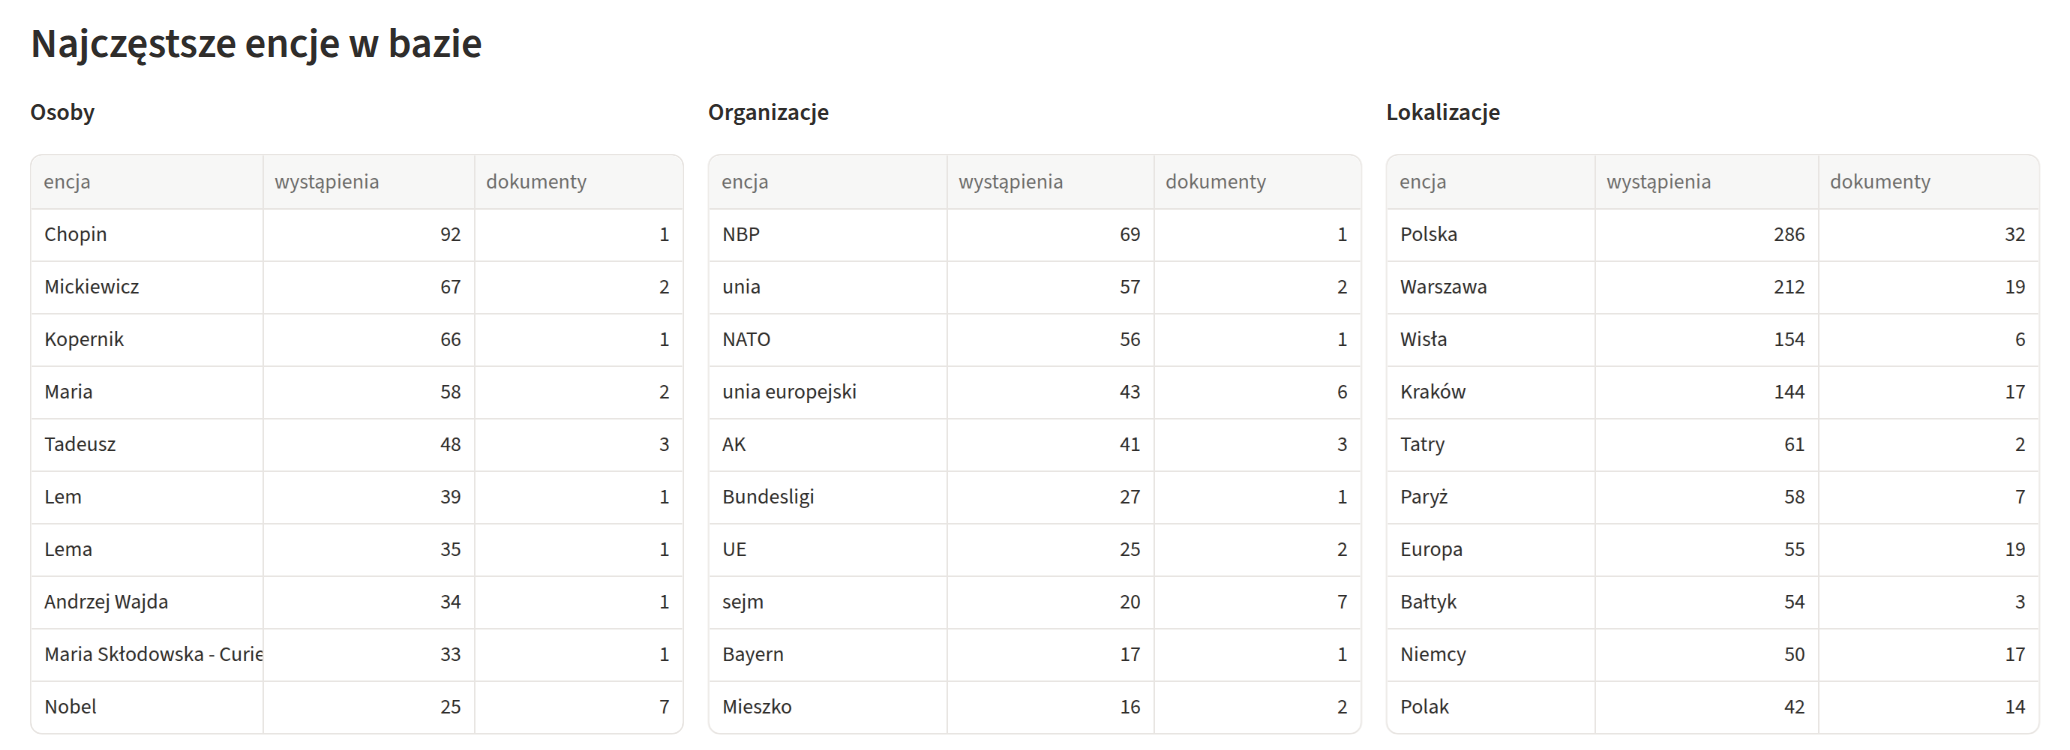
\includegraphics[width=\textwidth]{p2_gui_najczestsze.png}\\[0.3em]
    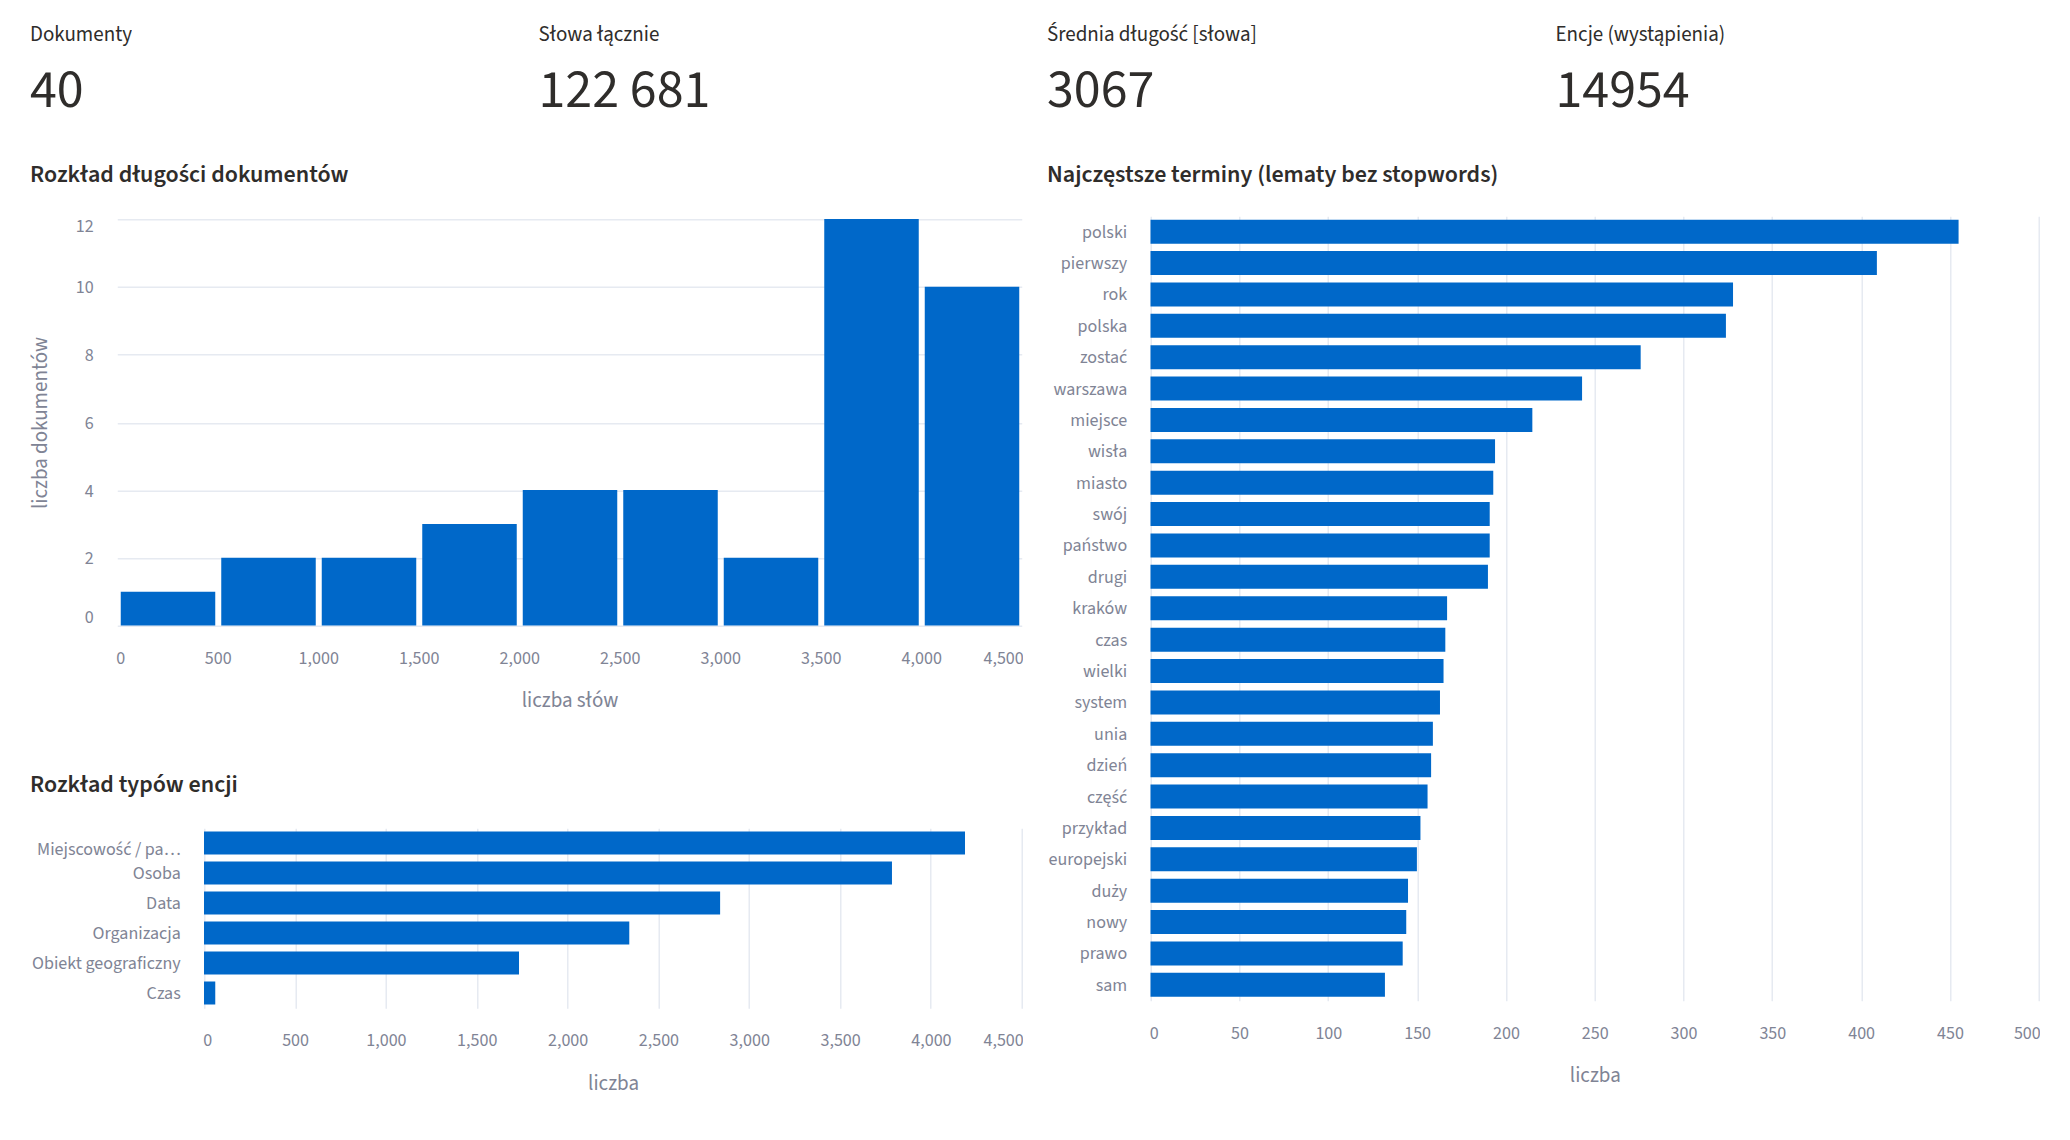
\includegraphics[width=\textwidth]{p2_gui_statystyki.png}
  \end{columns}
\end{frame}

\begin{frame}{Wnioski i ograniczenia}
  \begin{itemize}
    \item słowa kluczowe -- gdy znamy dokładną nazwę; TF-IDF -- gdy liczy się odmiana i rzadkie
          słowa; semantyczne -- gdy opisujemy temat własnymi słowami
    \item metody zgadzają się co do najlepszego dokumentu, ale nie co do reszty listy
          (średni Jaccard@5 od 0,28 do 0,52)
    \item lematyzacja jest kluczowa dla polskiego, ale myli się przy rzadkich nazwach własnych
    \item NER (NKJP) oznacza przymiotniki (,,polski'') jako miejsca, odmienia nazwiska niekonsekwentnie
    \item korpus mały i zróżnicowany -- na większym, jednorodnym różnice między metodami byłyby większe
  \end{itemize}
\end{frame}

\end{document}
